\part{Referenciais teóricos}

\chapter{Linguagens e gramáticas}
Uma linguagem é um conjunto arbitrário de cadeias - palavras - sobre um alfabeto \cite{lang}.
Uma das opções para a representação finita de uma linguagem é a utilização de uma gramática.
A noção formal de gramática foi introduzida por Noam Chomsky na década de 50. Uma gramática é definida como uma tupla que contém: 
um conunto finito de símbolos terminais, um conjunto finito de símbolos não-terminais, um estado inicial (pertencente ao conjunto dos símbolos não-terminais) e 
um conjunto finito de produções. Os conjuntos de símbolos terminais e não-terminais são disjuntos, ou seja, não possuem elementos em comum. \cite{gram}

\section{Classificação de Chomsky}
Toda gramática pode ser classificada de acordo com a Classificação de Chomsky onde toda gramática é pelo menos uma Gramática com Estrutura de Frase. A classe seguinte é um subconjunto da anterior e contém as Gramáticas Sensíveis ao Contexto. A classe das Gramáticas Livres de Contexto é novamente um subconjunto da classe anterior, assim como a ultima classe das Gramáticas Regulares é um subconjunto desta. A figura a seguir expressa a hierarquia existente entre as classes. A Classificação de Chomsky leva em conta como são as produções da gramática.

	
\begin{figure}[H]
	\caption{\label{gram_cls}Classes da Classificação de Chomsky e sua hierarquia}
	\begin{center}
	    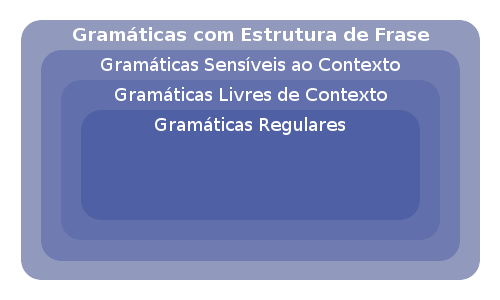
\includegraphics[scale=0.5]{driagrama_classes_gramaticas.png}
	\end{center}
	\legend{Fonte: Produzido pelo autor}
\end{figure}

Lembrando que as gramáticas são compostas por: um conjunto finito de símbolos não-terminais $N$, um conjunto finito de símbolos terminais $T$, um conjunto de produções $P$ e um símbolo inicial $\sigma$. A intersecção entre os conjuntos de símbolos não terminais e terminais deve ser vazia. O conjuto de produções é um subconjunto de todas as produções possíveis, o produto cartesiano de: todas as palavras geradas com símbolos não-terminais e terminais contendo pelo menos um símbolo não terminal (lado esquerdo da produção); todas as palavras geradas com símbolos não-terminais e terminais. O símbolo inicial deve pertencer ao conunto dos símbolos não terminais. Nas definições a seguir $\lambda$ denota a palavra nula. \cite{chomClass}

\subsection{Gramáticas com Estrutura de Frase}
A gramática é com Estrutura de Frase se todas as produções são da forma:

$\alpha \to \delta$, onde $\alpha \in (N \cup T)$* - $T$*, $\delta \in (N \cup T)$*.

\subsection{Gramáticas Sensíveis ao Contexto}
A gramática é Sensível ao Contexto se todas as produções são da forma:

$\alpha A\beta \to \alpha \delta \beta$, onde $\alpha,\beta \in (N \cup T)$*$, A \in N, \delta \in (N \cup T)$* - \{$\lambda$\}.

\subsection{Gramáticas Livres de Contexto}
A gramática é Livre de Contexto se todas as produções são da forma:

$A \to \delta$, onde $A \in N, \delta \in (N \cup T)$*.

\subsection{Gramáticas Regulares}
A gramática é Regular se todas as produções são da forma:

$A \to a$ ou $A \to aB$ ou $A \to \lambda$.

\chapter{Operações no Conjunto dos Números Inteiros}

O Conjunto dos Números Inteiros é fechado sob as operações de soma, subtração e multiplicação, isto significa que para qualquer uma destas operações o resultado é um número inteiro caso os operandos também sejam, mas não somente. A tabela a seguir apresenta exemplos para as propriedades comutativa e associativa das operações de soma e multiplicação.

\begin{table}[htb]
\IBGEtab{%
  \caption{Propriedades associativa e comutativa da soma e multiplicação sobre os Números Inteiros.}%
  \label{tabela-ibge}
}{%
  \begin{tabular}{ccc}
  \toprule
   Propriedade comutativa (adição/subtração) & $a+b=b+a$ & $ab=ba$ \\
  \midrule 
   Propriedade associativa (adição/subtração) & $(a+b)+c=a+(b+c) $ & $(ab)c=a(bc)$ \\
  \bottomrule
\end{tabular}%
}{%
  \fonte{Produzido pelo autor.}%
  }
\end{table}

A propriedade comutativa garante que a alteração da ordem dos operandos da operação não altera o seu resultado. A propriedade associativa diz respeito à mais de uma operação e garante que a ordem em que as operações são resolvidas não altera o resultado final das operações combinadas - na tabela apresentada anteriormente os parênteses não são necessários já que não existe precedência entre as operações (característica da operação associativa) e estão presentes apenas para explicitar a ordem de resolução.

\chapter{Árvores binárias ordenadas e rotações}
Uma árvore binária é uma coleção de dois tipos de nós, externos e internos, e três tipos de relações entre estes nós: pai, filho à esquerda e filho à direita. Todos os nós têm um nó pai, exceto um que é chamado de raíz. Os nós externos não possuem nós filhos, ao contrário dos nós internos que possuem dois nós filhos, um à esquerda e o outro da direita.

Árvores binárias são utilizadas em aplicações relacionadas a computador para guardar uma coleção de informações de forma ordenada, a ordem das informações é representada pela ordem simétrica dos nós. A ordem simétrica dos nós pode ser obtida utilizando o seguinte algoritmo recursivo: Se o nó é um nó interno passe pela subárvore à esquerda em ordem simétrica, passe pelo próprio nó e em seguida passe pela subárvore à direita em ordem simétrica. Se o nó é externo apenas passe por ele. A ordem de passagem dos nós é chamda de permutação de ordem simétrica dos nós ou apenas ordem simétrica dos nós. \cite{binTree}



\begin{figure}[H]
	\caption{\label{gram_cls}Diagrama sobre rotação de árvores binárias ordenadas}
	\begin{center}
	    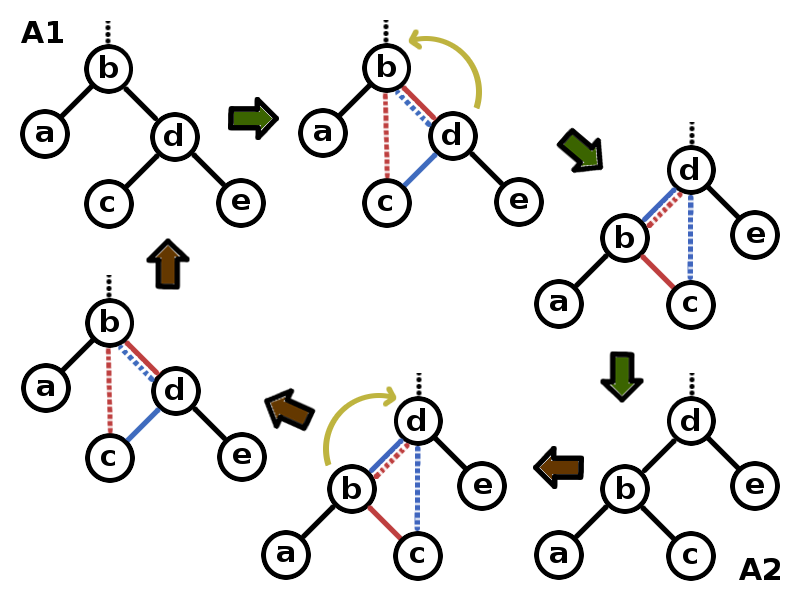
\includegraphics[scale=0.4]{tree_rotations.png}
	\end{center}
	\legend{Fonte: Produzido pelo autor}
\end{figure}

A rotação é uma operação que transforma uma árvore binária em outra mantendo a ordem simétrica dos nós. Em uma árvore de tamanho $n$ existem $n-1$ rotações possíveis \cite{binTree}. O diagrama contido na Figura 3 mostra graficamente como as rotações anti-horária e horária acontecem. A rotação anti-horária é explicada no fluxo por meio das setas verdes, que começa na árvore A1 e termina na árvore A2. A rotação horária de uma forma simétrica começa na árvore A2 e termina na árvore A1, as setas marrons representam o fluxo. As setas amarelas mostram o sentido das rotações executadas.

A rotação horária parte da árvore A2. A árvore seguinte mostra que o nó b, que inicialmente tem como filho direito o nó c, terá em seguida o nó d como seu filho direito. O filho esquerdo do nó d será alterado de nó b para nó c. A possível relação entre o nó d e o seu nó pai será passada para o nó b. Em seguida observamos como linhas contínuas as novas ligações e como tracejadas as antigas. Por fim chegamos a árvore A1 que é o resultado final da rotação horária sobre o nó d da árvore A2.

A rotação anti-horária é um processo simétrico à rotação horária. A sequência expressa pelas setas verdes, de A1 até A2, explica a transformação da mesma forma como a sua transformação inversa explicada no tópico anterior sendo assim não será explicada em detalhes.

\chapter{Números de Catalan}
Os números de Catalan aparecem em probelmas de enumeração de árvores como no problema de divisão dos polígonos de Euler. O $n$-ésimo número de Catalan pode ser obtido a partir da expressão $\frac{1}{n+1} \binom{2n}{n} $ \cite{wolfram}. Os dez primeiros números da sequência, começando com $n = 0$, são: 1, 1, 2, 5, 14, 42, 132, 429, 1430, 4862.

Os números de Catalan aparecem em diversos problemas, entre eles o problema das Ordens de Mutiplicação.
Este problema se refere a uma sucessão de $n$ multiplicações onde a ordem dos $n+1$ operandos não pode ser alterada. De acordo com a expressão apresentanda anteriormente a solução é o n-ésimo elemento do conjunto dos números de Catalan \cite{catNum}.
